\section{Density animation and export}

\subsection{Animation purpose}

A static Percepta image asks the observer to change viewing distance or zoom. Density animation performs a related transformation in time. It changes the spatial scale of the geometry while retaining the same source and rendering family. A sparse opening frame foregrounds the construction; a denser frame carries more source detail. The animation can therefore reveal how the illusion is built.

\begin{figure}[H]
  \centering
  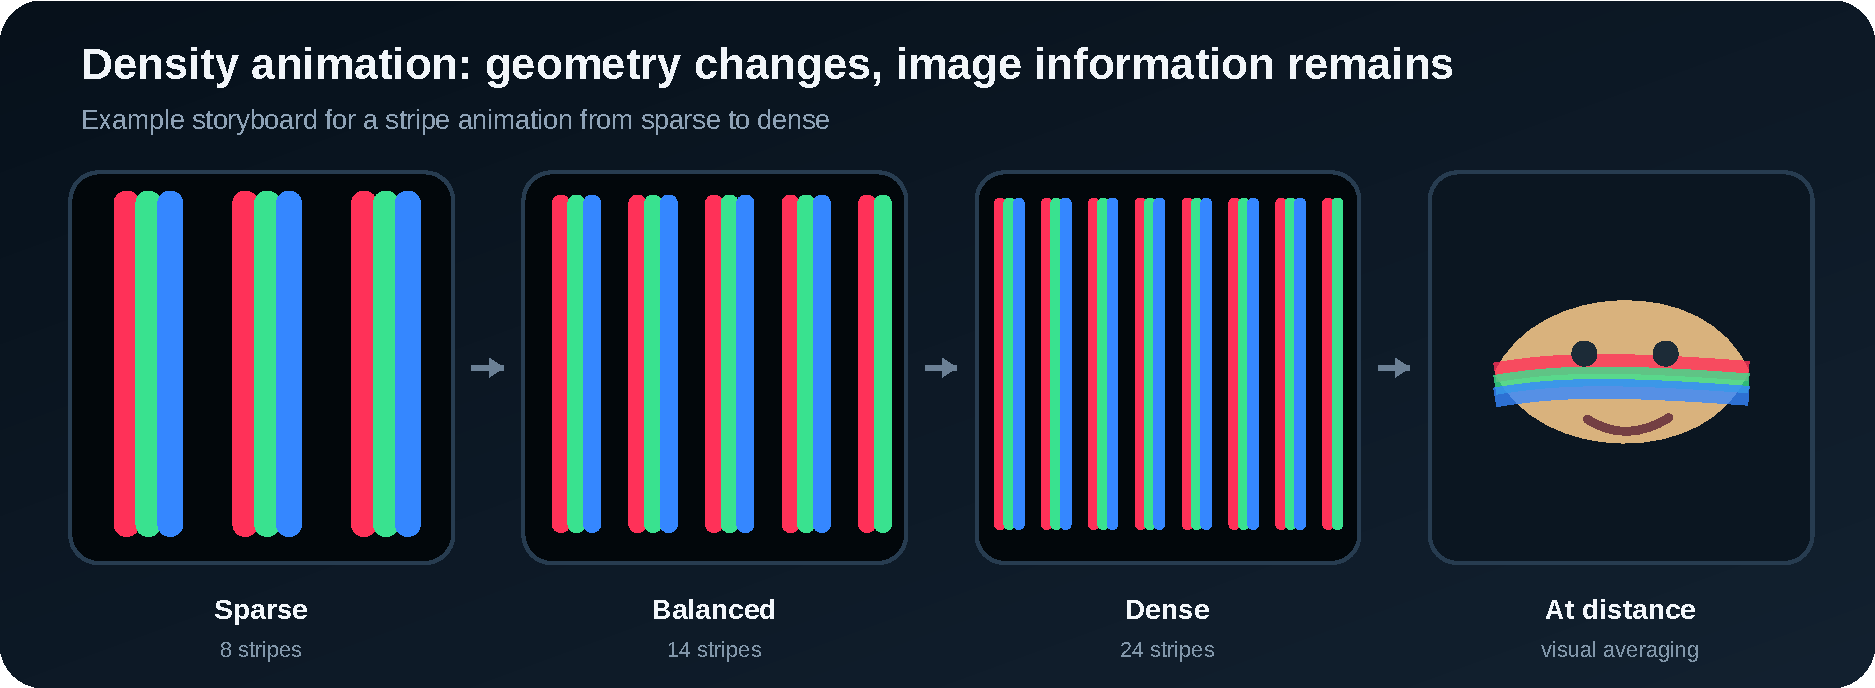
\includegraphics[width=0.92\textwidth]{build-assets/density-animation.pdf}
  \caption{Storyboard of a stripe-density animation. The application interpolates the active density parameter, not the source image.}
  \label{fig:animation}
\end{figure}

\subsection{Time normalisation}

Let the requested duration be $T$ seconds and the time of a frame be $t\in[0,T]$. Normalised time is

\begin{equation}
u=\clamp\!\left(\frac{t}{T},0,1\right).
\label{eq:normtime}
\end{equation}

An easing function $E(u)$ maps this interval to an interpolation phase. Linear interpolation uses

\begin{equation}
E_{\mathrm{lin}}(u)=u.
\end{equation}

A smoothstep easing with zero first derivative at both ends is

\begin{equation}
E_{\mathrm{smooth}}(u)=3u^2-2u^3.
\label{eq:smoothstep}
\end{equation}

A stronger quintic smoother is

\begin{equation}
E_{\mathrm{smoother}}(u)=6u^5-15u^4+10u^3.
\label{eq:smootherstep}
\end{equation}

The user-facing easing selector can expose one or more of these choices. Linear motion makes parameter speed constant; smooth easing makes the start and end less abrupt.

\subsection{Parameter interpolation}

For start value $p_0$ and end value $p_1$,

\begin{equation}
p(t)=p_0+\left(p_1-p_0\right)E\!\left(\frac{t}{T}\right).
\label{eq:parameterinterp}
\end{equation}

Stripe counts must be integer-valued, so the rendered count is

\begin{equation}
N(t)=\max\!\left(1,\operatorname{round}[p(t)]\right).
\label{eq:integeranim}
\end{equation}

Dot and turn spacing can remain real-valued until geometry is rasterised. This produces smoother animation than rounding spacing to integer pixels at every frame.

For halftone and spiral examples, animation commonly proceeds from a large spacing to a small spacing. Although the numeric value decreases, geometric density increases.

\subsection{Ping-pong phase}

Ping-pong playback traverses the range forward and then backward. For a repeating phase $u\in[0,1)$, a triangular phase is

\begin{equation}
u_{\triangle}=1-\left|2u-1\right|.
\label{eq:trianglephase}
\end{equation}

The animated parameter becomes

\begin{equation}
p_{\mathrm{pp}}(t)=p_0+\left(p_1-p_0\right)E(u_{\triangle}).
\end{equation}

If the exported duration $T$ is intended to include a full forward-and-back cycle, $u$ should span the triangle once over $T$. If $T$ describes only the forward leg, the full ping-pong duration is $2T$. The interface and export metadata should use one convention consistently.

\subsection{Frame rate and frame count}

At frame rate $F$ frames per second, a practical inclusive frame count is

\begin{equation}
N_f=\left\lfloor TF\right\rfloor+1.
\label{eq:framecount}
\end{equation}

Frame times can be defined by

\begin{equation}
t_k=\frac{k}{N_f-1}T,
\qquad k=0,1,\ldots,N_f-1.
\label{eq:frametimes}
\end{equation}

This includes the exact start and end states. For seamless looping, duplicating the terminal frame may cause a visible pause. Loop export can omit one duplicate endpoint or use timing metadata to maintain constant motion.

The raw uncompressed memory required to hold all RGB frames is approximately

\begin{equation}
M_{\mathrm{anim}}=3WHN_f\ \text{bytes}
\label{eq:animmemory}
\end{equation}

for 8-bit RGB. A 1600 px square, four-second animation at 12 FPS contains about 49 frames and would require approximately 376 MB if every frame were retained uncompressed. Streaming frames directly to the encoder is therefore preferable.

\subsection{Recommended animation ranges}

The following ranges are designed to show a meaningful transition without passing through excessively sparse or computationally wasteful states.

\begin{table}[H]
\centering
\caption{Reference density animation ranges at 1600 px.}
\begin{tabularx}{\textwidth}{>{\bfseries}l c c >{\raggedright\arraybackslash}X}
\toprule
Pattern & Start & End & Interpretation \\
\midrule
Vertical stripes & 8 & 24 & Threefold increase in carrier count \\
Horizontal stripes & 8 & 24 & Threefold increase in carrier count \\
Diagonal stripes & 10 & 28 & Denser range compensates for projected span \\
Halftone & 24 px & 7 px & Coarse dots become a detailed screen \\
Hexagonal halftone & 24 px & 7 px & Coarse triangular lattice becomes dense \\
Spiral stripes & 24 px & 6 px & Widely spaced turns tighten around the image \\
\bottomrule
\end{tabularx}
\end{table}

At higher output sizes, these values can be adaptively scaled using Equations~\eqref{eq:adaptivecount} and \eqref{eq:adaptivespacing}.

\subsection{Preview, playback and saving}

The animation controls serve distinct purposes:

\begin{itemize}
  \item \control{Preview} prepares or displays a reduced-resolution sequence for rapid evaluation.
  \item \control{Play} advances frames from the current position.
  \item \control{Pause} retains the current frame and allows playback to resume.
  \item \control{Stop} returns to a defined initial state.
  \item \control{Save} renders the requested output resolution and passes frames to the selected encoder.
\end{itemize}

Preview should prioritise responsiveness; final save should prioritise geometric and colour fidelity. A reduced preview can use lower output size or fewer frames, provided the interface clearly indicates that final export is rendered separately.

\subsection{Still-image export formats}

\subsubsection{PNG}

PNG is a lossless raster format suitable for the web, presentations and general image workflows. It preserves narrow coloured structures without JPEG blocking or chroma subsampling. File size can be large for detailed RGB patterns because the geometry contains many sharp colour transitions.

\subsubsection{TIFF}

TIFF is appropriate for high-resolution masters and print workflows. Depending on the writer, it can store lossless compression, metadata and higher bit depth. A print provider may prefer TIFF when the image is ultimately rasterised.

\subsubsection{SVG}

SVG represents geometric primitives as vectors. It is valuable for stripes, circles and spiral paths because the result can be scaled without pixelation. However, file size and rendering complexity can become high when every small dot or path segment is represented separately. Effects implemented only in raster form must either be approximated or embedded as raster content.

\subsubsection{PDF}

PDF is convenient for page-based distribution and professional printing. Vector-capable renderers can retain scalable geometry; raster output can also be embedded at a controlled physical size. The PDF page and artwork dimensions should be set intentionally rather than relying on a viewer's default scaling.

\subsection{Physical print size and raster resolution}

If the raster width is $W$ pixels and the print width is $S$ inches, the effective pixel density is

\begin{equation}
\mathrm{PPI}=\frac{W}{S}.
\label{eq:ppi}
\end{equation}

Conversely,

\begin{equation}
S=\frac{W}{\mathrm{PPI}}.
\end{equation}

A 4000 px output printed at 300 PPI is approximately 13.3 inches (33.9 cm) wide. At 200 PPI it is 20 inches (50.8 cm) wide. Geometric art can often tolerate lower PPI than photography, but thin RGB gaps must remain resolvable by the printer.

The physical period of a $P$-pixel pattern element is

\begin{equation}
p_{\mathrm{mm}}=25.4\frac{P}{\mathrm{PPI}}.
\label{eq:physicalperiod}
\end{equation}

This quantity, together with viewing distance, determines visual angle through Equation~\eqref{eq:angularperiod}.

\subsection{Colour management and printing}

Percepta is based on additive RGB mixing on screen. Printing uses subtractive inks and introduces dot gain, paper colour, ink limits and a device profile. A printed result can therefore differ from its emissive display preview.

Recommended practice:

\begin{enumerate}
  \item retain an RGB master and avoid repeated format conversions;
  \item use a colour-managed application for proofing;
  \item ask the printer for the intended ICC profile and rendering conditions;
  \item make a small physical proof at final scale;
  \item verify that the thinnest coloured structures do not disappear or merge;
  \item disable uncontrolled ``photo enhancement'' in consumer printer drivers.
\end{enumerate}

\begin{warningbox}
An SVG or PDF is not automatically print-safe. Vector geometry can be thinner than the output device can reproduce, and saturated RGB colours may lie outside the printer gamut. Physical proofing remains essential for important work.
\end{warningbox}


